\documentclass[border=4pt]{standalone}
\usepackage[T1]{fontenc}
\usepackage{lmodern}
\usepackage{amsmath}
\usepackage{pgfplots}
\pgfplotsset{compat=1.18}
\usepgfplotslibrary{groupplots,fillbetween}
\usetikzlibrary{calc,arrows.meta}
% one colour per kind of method, the same in every figure (Okabe-Ito)
\definecolor{neur}{HTML}{D55E00}   % neurons chosen by attribution
\definecolor{dirc}{HTML}{009E73}   % directions from the weird-vs-normal contrast
\definecolor{read}{HTML}{0072B2}   % readout methods and interventions chosen from readouts
\definecolor{pers}{HTML}{CC79A7}   % Assistant Axis / persona
\definecolor{ctrl}{HTML}{8C8C8C}   % random controls
\definecolor{meas}{HTML}{E69F00}   % measured outcome
\definecolor{ink}{HTML}{222222}
\pgfplotsset{
  every axis/.append style={clip=false, font=\small, axis line style={black!55}, tick style={black!55}, tick align=outside,
    label style={font=\small}, tick label style={font=\footnotesize}, title style={font=\small, align=center}},
  grid style={black!9, line width=0.4pt},
  every axis legend/.append style={font=\footnotesize, draw=none, fill=none},
  ci/.style={/pgfplots/error bars/x dir=both, /pgfplots/error bars/x explicit, /pgfplots/error bars/error bar style={line width=0.8pt}, /pgfplots/error bars/error mark=none},
  yci/.style={/pgfplots/error bars/y dir=both, /pgfplots/error bars/y explicit, /pgfplots/error bars/error bar style={line width=0.8pt}, /pgfplots/error bars/error mark=none},
}

\begin{document}
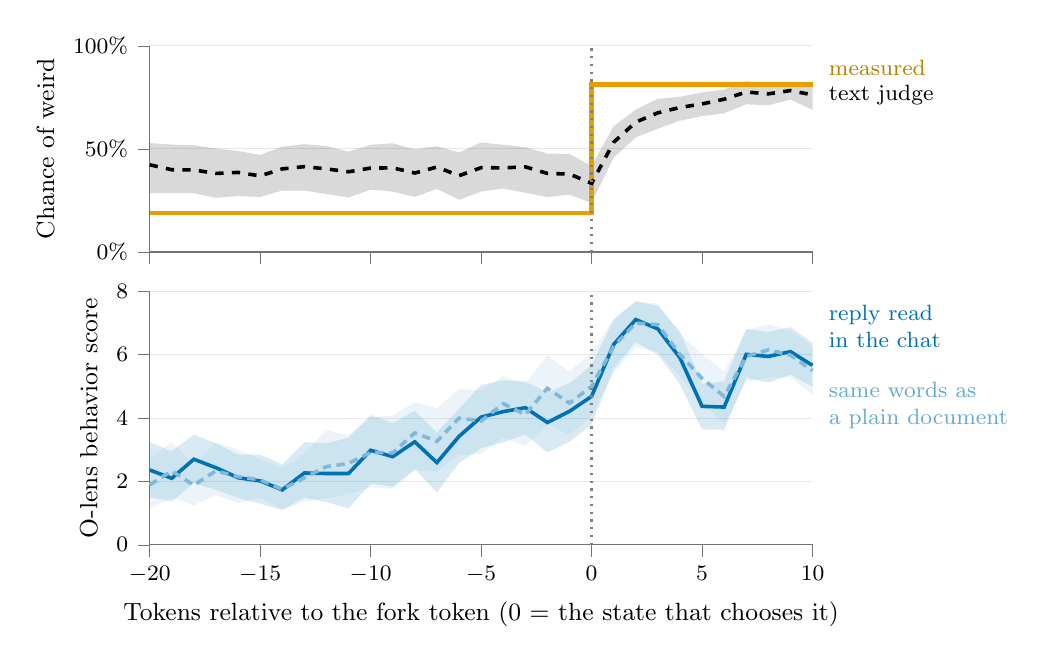
\begin{tikzpicture}
\begin{groupplot}[group style={group size=1 by 2, vertical sep=0.5cm, x descriptions at=edge bottom}, width=10cm, xmin=-20, xmax=10, xtick={-20,-15,-10,-5,0,5,10}, axis x line*=bottom, axis y line*=left, ymajorgrids]
\nextgroupplot[height=4.2cm, ymin=0, ymax=1, ytick={0,0.5,1}, yticklabels={0\%,50\%,100\%}, ylabel={Chance of weird}]
\addplot[meas, line width=1.6pt, const plot] coordinates {(-20,0.188) (0,0.812) (10,0.812)};
\addplot[name path=ut, draw=none] coordinates {(-20,0.528) (-19,0.521) (-18,0.518) (-17,0.502) (-16,0.490) (-15,0.471) (-14,0.511) (-13,0.523) (-12,0.514) (-11,0.487) (-10,0.520) (-9,0.527) (-8,0.498) (-7,0.513) (-6,0.483) (-5,0.531) (-4,0.520) (-3,0.508) (-2,0.477) (-1,0.476) (0,0.417) (1,0.610) (2,0.691) (3,0.743) (4,0.753) (5,0.774) (6,0.788) (7,0.830) (8,0.813) (9,0.823) (10,0.811)};\addplot[name path=dt, draw=none] coordinates {(-20,0.285) (-19,0.287) (-18,0.285) (-17,0.263) (-16,0.271) (-15,0.267) (-14,0.298) (-13,0.298) (-12,0.281) (-11,0.264) (-10,0.302) (-9,0.293) (-8,0.267) (-7,0.306) (-6,0.253) (-5,0.293) (-4,0.308) (-3,0.287) (-2,0.266) (-1,0.278) (0,0.238) (1,0.458) (2,0.556) (3,0.598) (4,0.637) (5,0.659) (6,0.673) (7,0.716) (8,0.712) (9,0.739) (10,0.690)};\addplot[black, fill opacity=0.15] fill between[of=ut and dt];\addplot[black, line width=1.3pt, dashed] coordinates {(-20,0.423) (-19,0.399) (-18,0.398) (-17,0.381) (-16,0.386) (-15,0.369) (-14,0.403) (-13,0.414) (-12,0.403) (-11,0.389) (-10,0.407) (-9,0.408) (-8,0.383) (-7,0.412) (-6,0.370) (-5,0.409) (-4,0.408) (-3,0.413) (-2,0.381) (-1,0.378) (0,0.333) (1,0.532) (2,0.630) (3,0.675) (4,0.701) (5,0.718) (6,0.741) (7,0.776) (8,0.767) (9,0.783) (10,0.762)};
\draw[black!50, dotted, line width=0.8pt] (axis cs:0,0) -- (axis cs:0,1);
\node[font=\footnotesize, anchor=west] at (axis cs:10.3,0.762) {text judge};
\node[font=\footnotesize, meas!80!black, anchor=west] at (axis cs:10.3,0.892) {measured};
\nextgroupplot[height=4.8cm, ymin=0, ymax=8, ytick={0,2,4,6,8}, ylabel={O-lens behavior score}, xlabel={Tokens relative to the fork token (0 = the state that chooses it)}]
\addplot[name path=ul, draw=none] coordinates {(-20,3.241) (-19,2.951) (-18,3.483) (-17,3.200) (-16,2.850) (-15,2.850) (-14,2.534) (-13,3.234) (-12,3.200) (-11,3.383) (-10,4.100) (-9,3.834) (-8,4.235) (-7,3.547) (-6,4.297) (-5,5.047) (-4,5.188) (-3,5.156) (-2,4.806) (-1,5.101) (0,5.676) (1,7.109) (2,7.696) (3,7.533) (4,6.739) (5,5.077) (6,5.163) (7,6.805) (8,6.718) (9,6.870) (10,6.370)};\addplot[name path=dl, draw=none] coordinates {(-20,1.500) (-19,1.366) (-18,1.950) (-17,1.733) (-16,1.483) (-15,1.299) (-14,1.099) (-13,1.483) (-12,1.350) (-11,1.150) (-10,1.933) (-9,1.833) (-8,2.389) (-7,1.656) (-6,2.578) (-5,3.046) (-4,3.234) (-3,3.483) (-2,2.916) (-1,3.249) (0,3.793) (1,5.554) (2,6.402) (3,6.010) (4,5.065) (5,3.641) (6,3.630) (7,5.271) (8,5.119) (9,5.370) (10,4.989)};\addplot[read, fill opacity=0.15] fill between[of=ul and dl];\addplot[read, line width=1.3pt] coordinates {(-20,2.362) (-19,2.100) (-18,2.700) (-17,2.433) (-16,2.117) (-15,2.017) (-14,1.733) (-13,2.267) (-12,2.250) (-11,2.250) (-10,2.983) (-9,2.783) (-8,3.250) (-7,2.594) (-6,3.422) (-5,4.031) (-4,4.203) (-3,4.328) (-2,3.861) (-1,4.213) (0,4.685) (1,6.326) (2,7.109) (3,6.815) (4,5.902) (5,4.370) (6,4.348) (7,6.011) (8,5.946) (9,6.098) (10,5.663)};
\addplot[name path=ur, draw=none] coordinates {(-20,2.733) (-19,3.242) (-18,2.533) (-17,3.235) (-16,3.001) (-15,2.701) (-14,2.417) (-13,2.900) (-12,3.619) (-11,3.451) (-10,4.017) (-9,4.084) (-8,4.500) (-7,4.313) (-6,4.923) (-5,4.875) (-4,5.329) (-3,5.079) (-2,5.985) (-1,5.472) (0,6.076) (1,7.120) (2,7.674) (3,7.620) (4,6.642) (5,6.022) (6,5.467) (7,6.783) (8,6.957) (9,6.761) (10,6.261)};\addplot[name path=dr, draw=none] coordinates {(-20,1.143) (-19,1.482) (-18,1.250) (-17,1.566) (-16,1.316) (-15,1.483) (-14,1.116) (-13,1.366) (-12,1.465) (-11,1.616) (-10,1.815) (-9,1.765) (-8,2.350) (-7,2.312) (-6,2.844) (-5,2.859) (-4,3.390) (-3,3.109) (-2,3.796) (-1,3.472) (0,4.075) (1,5.424) (2,6.239) (3,6.087) (4,5.326) (5,4.511) (6,3.815) (7,5.141) (8,5.283) (9,5.282) (10,4.728)};\addplot[read!50, fill opacity=0.15] fill between[of=ur and dr];\addplot[read!50, line width=1.3pt, densely dashed] coordinates {(-20,1.893) (-19,2.328) (-18,1.883) (-17,2.333) (-16,2.150) (-15,2.050) (-14,1.750) (-13,2.117) (-12,2.467) (-11,2.567) (-10,2.917) (-9,2.900) (-8,3.533) (-7,3.266) (-6,4.000) (-5,3.906) (-4,4.453) (-3,4.109) (-2,4.938) (-1,4.472) (0,5.000) (1,6.261) (2,7.000) (3,6.946) (4,6.011) (5,5.250) (6,4.685) (7,5.946) (8,6.152) (9,5.989) (10,5.500)};
\draw[black!50, dotted, line width=0.8pt] (axis cs:0,0) -- (axis cs:0,8);
\node[font=\footnotesize, read, anchor=west, align=left] at (axis cs:10.3,6.9) {reply read\\in the chat};
\node[font=\footnotesize, read!60, anchor=west, align=left] at (axis cs:10.3,4.4) {same words as\\a plain document};
\end{groupplot}
\end{tikzpicture}
\end{document}
